\documentclass{article}
\usepackage{tikz}

\begin{document}

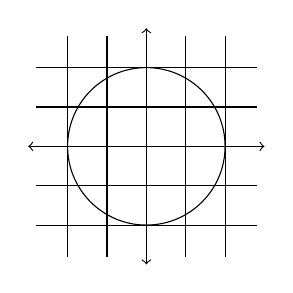
\begin{tikzpicture}
    \draw[<->] (-1.5,0) -- (1.5,0);
    \draw[<->] (0,-1.5) -- (0,1.5);
    \draw (0,0) circle [radius=1];
    \draw[step=0.5, thin] (-1.4,-1.4) grid (1.4,1.4);
\end{tikzpicture}

\newpage 

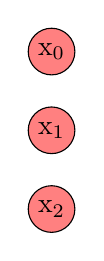
\begin{tikzpicture}[
    inputnode/.style={draw, circle, fill=red!50, inner sep=2pt},
]
     \node[inputnode] (x0) at (0, 1) {$\mathrm{x}_0$};
     \node[inputnode] (x1) at (0, 0) {$\mathrm{x}_1$};
     \node[inputnode] (x2) at (0, -1) {$\mathrm{x}_2$};
\end{tikzpicture}

\newpage 

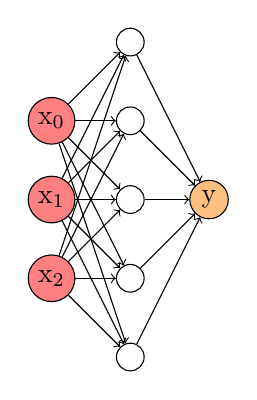
\begin{tikzpicture}[
    inputnode/.style={draw, circle, fill=red!50, inner sep=2pt},
    hiddenunit/.style={draw, circle, minimum size=10pt},
    outnode/.style={draw, circle, fill=orange!50, inner sep=2pt},
]
    \node[inputnode] (x0) at (0, 1) {$\mathrm{x}_0$};
    \node[inputnode] (x1) at (0, 0) {$\mathrm{x}_1$};
    \node[inputnode] (x2) at (0, -1) {$\mathrm{x}_2$};
    
    \node[hiddenunit] (h2) at (1, 2) {};
    \node[hiddenunit] (h1) at (1, 1) {};
    \node[hiddenunit] (h0) at (1, 0) {};
    \node[hiddenunit] (h3) at (1, -1) {};
    \node[hiddenunit] (h4) at (1, -2) {};
    
    \node[outnode] (y0) at (2, 0) {$\mathrm{y}$};

    \foreach \x in {x0, x1, x2} {
        \foreach \h in {h0, h1, h2, h3, h4} {
            \draw[->] (\x) -- (\h); 
        }
    }

    \foreach \h in {h0, h1, h2, h3, h4} {
        \draw[->] (\h) -- (y0); 
    }
    

\end{tikzpicture}
    

\newpage 

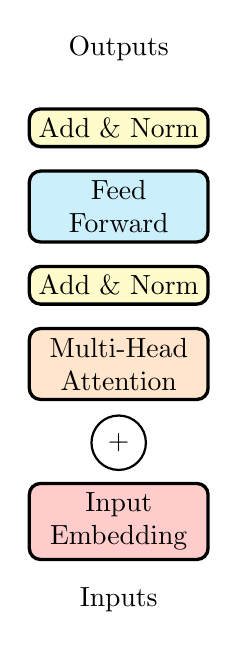
\begin{tikzpicture}[
    module/.style={draw, very thick, rounded corners, minimum width=15ex},
    embmodule/.style={module, fill=red!20},
    mhamodule/.style={module, fill=orange!20},
    lnmodule/.style={module, fill=yellow!20},
    ffnmodule/.style={module, fill=cyan!20},
    arrow/.style={-stealth', thick, rounded corners},
    ]
    \node (inputs) {Inputs};
    \node[above of=inputs, embmodule, align=center]
    (inputemb) {Input\\Embedding};
    \node[above of=inputemb, draw, thick, circle] (embplus)
    {$+$};
    \node[above of=embplus, mhamodule, align=center] (mha)
     {Multi-Head\\Attention};
    \node[above of=mha, lnmodule, align=center] (addnorm1)
    {Add \& Norm};
    \node[above of=addnorm1, ffnmodule, align=center] (ffn)
     {Feed\\Forward};
    \node[above of=ffn, lnmodule, align=center] (addnorm2)
    {Add \& Norm};
    \node[above of=addnorm2] (outputs) {Outputs};
\end{tikzpicture}

\end{document}
